% =============================================================================
% Agent-First Middleware for OLAP Systems
% SAO Workshop Paper
%
% Uses the ACM "sigconf" format consistent with the SAO paper venue.
% To compile: pdflatex paper && bibtex paper && pdflatex paper && pdflatex paper
% =============================================================================
\documentclass[sigconf, nonacm]{acmart}

% ---------------------------------------------------------------------------
% Packages
% ---------------------------------------------------------------------------
\usepackage{booktabs}          % Professional tables
\usepackage{multirow}          % Multi-row table cells
\usepackage{xcolor}            % Colors (for todo markers)
\usepackage{algorithm}         % Algorithm floats
\usepackage{algpseudocode}     % Pseudocode typesetting
\usepackage{listings}          % Code listings
\usepackage{subcaption}        % Sub-figures
\usepackage{graphicx}          % Graphics inclusion
\usepackage{xspace}            % Smart spacing after macros
\usepackage{enumitem}          % List customization
\usepackage{balance}           % Balance final page columns

% ---------------------------------------------------------------------------
% Custom commands
% ---------------------------------------------------------------------------
\newcommand{\todo}[1]{\textcolor{red}{\textbf{[TODO: #1]}}}
\newcommand{\sysname}{\textsc{AgentGate}\xspace}  % Change system name as desired
\newcommand{\ie}{\textit{i.e.}\xspace}
\newcommand{\eg}{\textit{e.g.}\xspace}
\newcommand{\etal}{\textit{et~al.}\xspace}

% ---------------------------------------------------------------------------
% Listings style for SQL / Python
% ---------------------------------------------------------------------------
\lstdefinestyle{sqlstyle}{
  language=SQL,
  basicstyle=\ttfamily\footnotesize,
  keywordstyle=\bfseries\color{blue!70!black},
  commentstyle=\color{green!50!black},
  stringstyle=\color{red!60!black},
  showstringspaces=false,
  frame=single,
  breaklines=true,
  captionpos=b
}

\lstdefinestyle{pythonstyle}{
  language=Python,
  basicstyle=\ttfamily\footnotesize,
  keywordstyle=\bfseries\color{blue!70!black},
  commentstyle=\color{green!50!black},
  stringstyle=\color{red!60!black},
  showstringspaces=false,
  frame=single,
  breaklines=true,
  captionpos=b
}

% ---------------------------------------------------------------------------
% Document metadata
% ---------------------------------------------------------------------------
\title{Agent-First Middleware for OLAP Systems: \\
       Intent-Based Access Control, Query Learning, and Schema Discovery}

\author{Mohit Tripathi}
\affiliation{%
  \institution{Bloomberg}
}
\email{mtripathi15@bloomberg.net}


% Add more authors as needed

% ---------------------------------------------------------------------------
\begin{document}
% ---------------------------------------------------------------------------

% =====================================================================
% ABSTRACT
% =====================================================================
\begin{abstract}
As LLM-powered agents become the dominant consumers of analytical data systems,
a fundamental mismatch emerges: OLAP databases were designed for human users who
craft careful queries, not for agents that issue hundreds of exploratory probes
per session. Liu \etal~\cite{liu2025sao} characterize agentic workloads by
four properties---\emph{scale}, \emph{heterogeneity}, \emph{redundancy}, and
\emph{steerability}---and call for redesigning data systems to be agent-first.

This work presents \sysname, a transparent middleware layer that sits between
LLM agents and OLAP databases.  \sysname introduces three mechanisms:
(1)~\emph{intent-based access control} that parses SQL ASTs to enforce policies
at the semantic level (\eg, allowing aggregations over sensitive columns while
blocking row-level access);
(2)~\emph{session-based query learning} that persists agent sessions as
embeddings and surfaces relevant past queries to new agents with similar
goals, enabling cross-task knowledge transfer; and
(3)~a curated \emph{explore endpoint} that provides schema metadata, column
semantics, access-level annotations, and sample queries, eliminating the
redundant schema-discovery queries that dominate agentic workloads.

\sysname is evaluated on a distributed ClickHouse cluster with two benchmark
tracks.
A \emph{security benchmark} (5~attack scenarios, 200~probes) shows that the
middleware blocks 67~additional attacks versus unprotected ClickHouse,
reducing PII leakage from 300 to~0 rows.
An \emph{agent-efficiency benchmark} (8~analytical tasks, 3~models, up to
10~sequential agents per task) demonstrates that the middleware reduces total
queries hitting the OLAP system by 74.5\% (200$\to$51) and eliminates all
95~schema-exploration queries.  An explore-endpoint ablation shows that
without the endpoint, task success drops from 100\% to 12.5\%, confirming
that the explore layer is the foundational enabler for policy-compliant agent
interactions.  Cross-task transfer experiments show that queries stored by
agents solving one task reduce queries for semantically related tasks by 90\%.
Agent capability matters: GPT-4o achieves 62.5\% accuracy in 1.1~queries on
average, GPT-4o-mini achieves 45.8\% in 3.5~queries, while Qwen-3.5 scores
25\% despite the same middleware support, indicating that agent-first
middleware amplifies model capability rather than leveling it.
\end{abstract}

\maketitle

% =====================================================================
% 1. INTRODUCTION
% =====================================================================
\section{Introduction}
\label{sec:intro}

The interface between data systems and their consumers is undergoing a
structural shift. Where human analysts once formulated precise SQL queries
informed by domain expertise and schema knowledge, LLM-powered agents now
interact with databases through iterative, exploratory probe
sequences~\cite{liu2025sao}. These agentic workloads differ qualitatively from
traditional analytics: they exhibit high \emph{scale} (hundreds of queries per
task), substantial \emph{heterogeneity} (mixing metadata exploration with
analytical computation), pervasive \emph{redundancy} (repeating similar
schema-discovery patterns across sessions), and latent
\emph{steerability} (responding to richer feedback than simple error
messages)~\cite{liu2025sao}.

This shift exposes three critical gaps in current OLAP architectures.

\paragraph{Security.}
Traditional role-based access control (RBAC)~\cite{sandhu1996rbac} operates at
the table or column level: a principal either can or cannot access a column.
But agentic intent is more nuanced. An agent computing \texttt{AVG(salary)
GROUP BY department} poses fundamentally different privacy risk than one
executing \texttt{SELECT name, salary FROM employees}---yet both access the
same column. Current systems cannot distinguish between these intents, forcing
administrators into a binary choice between permitting all access (risking PII
leakage) or blocking the column entirely (crippling legitimate analytics).

\paragraph{Resource governance.}
Unlike human analysts who self-regulate query frequency, agent swarms can flood
an OLAP cluster with hundreds of concurrent requests---mixing expensive
analytical scans with speculative exploration probes.  Most OLAP systems offer
per-user resource governors (max memory, max threads), but these are static
limits designed for tens of concurrent users, not for dynamically managing
thousands of agents.  There is no concept of binding an agent to a principal
identity across sessions, capping its concurrent queries, or throttling its
request rate with backoff signals.  Without such governance, a single
misconfigured agent loop can degrade query latency for the entire cluster.

\paragraph{Efficiency.}
Liu \etal~\cite{liu2025sao} observe that 80--90\% of agent queries in
text-to-SQL benchmarks are redundant schema-exploration
probes---\texttt{DESCRIBE TABLE}, \texttt{SHOW COLUMNS}, and speculative
\texttt{SELECT *} queries whose sole purpose is to map the schema landscape.
These probes consume tokens, exhaust rate limits, and inflate latency, yet
yield information the data system already possesses. No mechanism exists to
proactively surface this metadata in a form agents can directly consume.

\medskip
This work presents \sysname, a transparent middleware layer that addresses these
gaps without modifying the underlying OLAP engine.  \sysname contributes four
mechanisms:

\begin{enumerate}[leftmargin=*]
  \item \textbf{Intent-based access control} (\S\ref{sec:access}): SQL AST
        parsing with \texttt{sqlglot}~\cite{sqlglot2023} classifies query
        intent and enforces policies at the semantic level---allowing
        aggregations over sensitive columns while blocking row-level access
        to the same data.

  \item \textbf{Session-based query learning} (\S\ref{sec:learning}):
        Agent sessions are embedded and persisted in a vector store,
        enabling cross-agent and cross-task knowledge transfer.  Queries
        validated by one agent are surfaced to future agents with
        semantically similar goals.

  \item \textbf{Curated explore endpoint} (\S\ref{sec:explore}):
        Access-controlled schema metadata enriched with column semantics,
        access-level annotations, and sample queries eliminates redundant
        exploration.  Critically, the explore endpoint serves dual
        purpose: schema discovery \emph{and} policy guidance, teaching
        agents how to formulate compliant queries rather than merely
        blocking non-compliant ones.

  \item \textbf{Agent resource governance} (\S\ref{sec:governance}):
        Each agent is bound to a single principal with per-agent rate
        limits, concurrent query caps, and full audit logging---regardless
        of how many sessions or connections it opens.  Rate-limited
        requests receive \texttt{Retry-After} headers, enabling
        well-behaved agents to back off gracefully rather than overloading
        the cluster.
\end{enumerate}

By design, the middleware architecture places a protective layer between
agents and the OLAP cluster.  Every query passes through access control,
rate limiting, and audit logging before reaching the database---shielding
the cluster from both malicious and accidental abuse.  \sysname deploys as
an OLAP-compatible HTTP proxy, requiring zero changes to existing agent
tooling.  It is evaluated on a distributed ClickHouse cluster across two
benchmark tracks:

\begin{itemize}[leftmargin=*]
  \item A \emph{security benchmark} (5~attack scenarios, 200~probes) in
        which the middleware blocks 67~additional attacks and eliminates all
        PII leakage (300$\to$0~rows; \S\ref{sec:security-eval}).

  \item An \emph{agent-efficiency benchmark} (8~analytical tasks, 3~LLM
        models, up to 10~sequential agents) that reduces queries hitting the
        OLAP system by 74.5\% and eliminates all 95~schema-exploration
        queries (\S\ref{sec:agent-eval}).  An ablation study shows that
        removing the explore endpoint drops task success from 100\% to 12.5\%
        (\S\ref{sec:explore-ablation}), and cross-task transfer experiments
        demonstrate a 90\% query reduction when agents benefit from prior
        sessions on related tasks (\S\ref{sec:cross-task}).
\end{itemize}


% =====================================================================
% 2. BACKGROUND
% =====================================================================
\section{Background and Motivation}
\label{sec:background}

\subsection{Agentic Workload Characteristics}

Liu \etal~\cite{liu2025sao} analyze agent interactions with data systems on the
BIRD benchmark~\cite{li2024bird} and identify four distinguishing
characteristics of agentic workloads:

\begin{description}[leftmargin=*,labelwidth=1.5cm]
  \item[Scale.]
    Agents generate orders-of-magnitude more queries than human analysts per
    task, driven by iterative exploration and trial-and-error solution
    formulation.

  \item[Heterogeneity.]
    Agent probes span a wide spectrum: coarse-grained metadata discovery,
    partial query attempts, schema exploration, and final analytical
    computation. \todo{Add specific percentages from SAO paper Table~1.}

  \item[Redundancy.]
    Across sessions and agents, many probes access similar data or perform
    overlapping operations. Schema-discovery queries (\texttt{SHOW TABLES},
    \texttt{DESCRIBE}, \texttt{SELECT * LIMIT 5}) account for 80--90\% of
    total probes.

  \item[Steerability.]
    Unlike traditional query interfaces that return only results or errors,
    agents can consume and act on richer feedback---query suggestions,
    constraint explanations, and semantic metadata---if the data system provides
    it.
\end{description}

These characteristics motivate a middleware layer that addresses redundancy
through proactive metadata exposure, leverages steerability through structured
feedback, and imposes security constraints that understand agent intent rather
than merely restricting column access.

\subsection{Limitations of Existing Approaches}
\label{sec:limitations}

\paragraph{Text-to-SQL systems.}
Systems like DIN-SQL~\cite{pourreza2024dinsql} focus on translating natural
language to SQL with high accuracy. However, they treat the data system as a
black box and do not address the security or efficiency dimensions of agentic
interaction---an agent using DIN-SQL still needs schema discovery and still
lacks intent-aware access control.

\paragraph{Traditional access control.}
RBAC~\cite{sandhu1996rbac} and fine-grained access control
systems~\cite{rizvi2004extending} enforce policies at the row, column, or
view level. These mechanisms cannot distinguish between query intents over the
same column. \todo{Add specific example showing RBAC failure mode.}

\paragraph{Query guardrails.}
LLM guardrail frameworks~\cite{rebedea2023nemo} operate at the prompt level,
filtering natural-language inputs before they reach the model. They do not
inspect generated SQL and cannot enforce data-level policies.
\todo{Expand with additional guardrail systems.}


% =====================================================================
% 3. SYSTEM ARCHITECTURE
% =====================================================================
\section{System Architecture}
\label{sec:architecture}

Figure~\ref{fig:architecture} shows the \sysname architecture. The middleware
interposes between LLM agents and a ClickHouse~\cite{clickhouse2024} OLAP
backend via a transparent HTTP proxy. Three services compose the middleware
layer.

\begin{figure}[t]
  \centering
  % 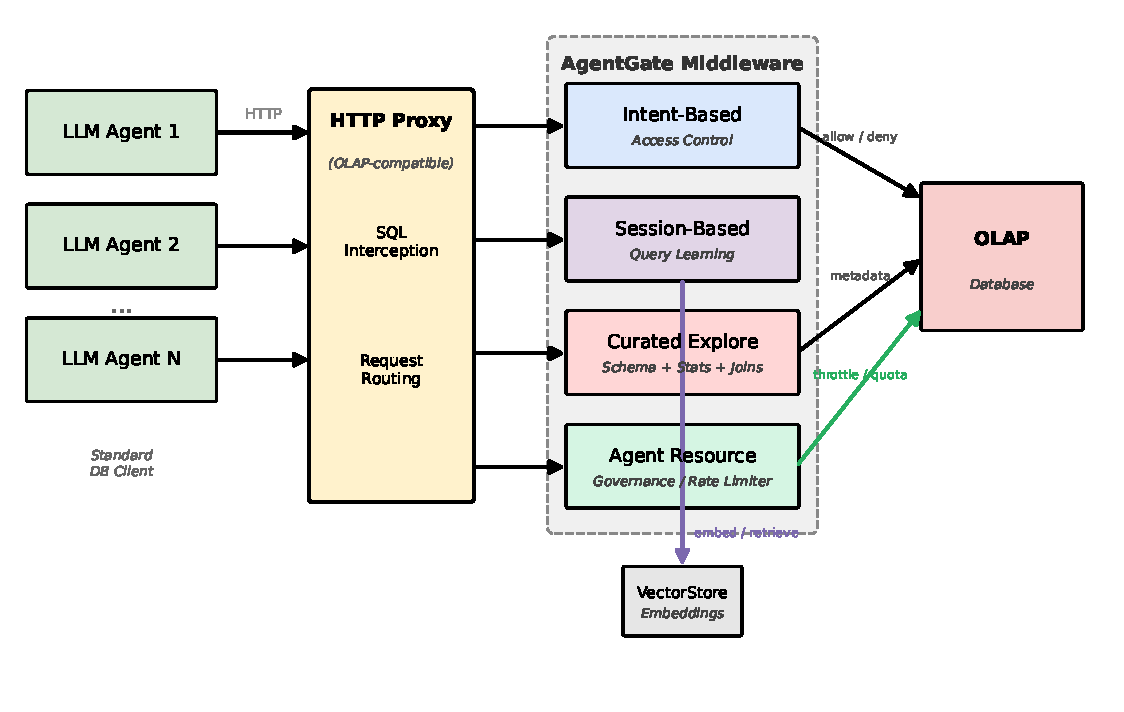
\includegraphics[width=\columnwidth]{figures/architecture.pdf}
  \fbox{\parbox{0.9\columnwidth}{\centering\vspace{3em}
    \todo{Insert architecture diagram showing:\\
    Agent $\rightarrow$ HTTP Proxy $\rightarrow$ [Access Control | Query Learning | Explore] $\rightarrow$ ClickHouse}
  \vspace{3em}}}
  \caption{%
    \sysname architecture. The middleware sits between LLM agents and
    ClickHouse, providing intent-based access control, session-based query
    learning, and a curated explore endpoint. Existing tools
    (\texttt{clickhouse\_connect}) connect through the proxy unmodified.
  }
  \label{fig:architecture}
\end{figure}

% ----- 3.1 Access Control -----
\subsection{Intent-Based Access Control}
\label{sec:access}

Traditional access control answers a binary question: \emph{can this principal
access this column?} \sysname asks a richer question: \emph{what does this
principal intend to do with this column, and is that intent permitted?}

\paragraph{Query intent classification.}
\sysname parses every incoming SQL statement into an AST using
\texttt{sqlglot}~\cite{sqlglot2023} and classifies the query into one of three
intent categories:

\begin{itemize}[leftmargin=*]
  \item \texttt{SELECT\_ROW}: Row-level data retrieval. The query returns
        individual records from sensitive columns without aggregation.
  \item \texttt{AGGREGATE}: Statistical computation. The query applies
        aggregate functions (\texttt{AVG}, \texttt{SUM}, \texttt{COUNT}, etc.)
        over sensitive columns, returning only summary statistics.
  \item \texttt{DDL/DML}: Schema modification or data mutation
        (\texttt{CREATE}, \texttt{INSERT}, \texttt{UPDATE}, \texttt{DELETE}).
\end{itemize}

\paragraph{Resource registry.}
Every column in the schema is annotated with a sensitivity classification
drawn from a controlled vocabulary:

\begin{itemize}[leftmargin=*]
  \item \texttt{PII} --- Personally identifiable information (\eg, names,
        emails, SSNs).
  \item \texttt{FINANCIAL} --- Revenue, salary, pricing data.
  \item \texttt{BUSINESS\_SECRET} --- Proprietary metrics, internal
        classifications.
  \item \texttt{SAFE} --- Non-sensitive columns (\eg, timestamps, categories).
\end{itemize}

\paragraph{Policy enforcement.}
The access control service composes intent classification with resource
sensitivity to enforce policies. For example, a default policy permits
\texttt{AGGREGATE} queries over \texttt{PII} columns (revealing
\texttt{AVG(salary)} but not individual salaries) while blocking
\texttt{SELECT\_ROW} access. Algorithm~\ref{alg:access} formalizes this logic.

\begin{algorithm}[t]
\caption{Intent-Based Access Control}
\label{alg:access}
\begin{algorithmic}[1]
\Require SQL query $q$, agent role $r$, resource registry $\mathcal{R}$, policy set $\mathcal{P}$
\Ensure \textsc{Allow} or \textsc{Deny} with explanation
\State $\mathit{ast} \gets \textsc{Parse}(q)$ \Comment{sqlglot AST}
\State $\mathit{intent} \gets \textsc{ClassifyIntent}(\mathit{ast})$
        \Comment{\texttt{SELECT\_ROW} | \texttt{AGGREGATE} | \texttt{DDL\_DML}}
\State $\mathit{cols} \gets \textsc{ExtractColumns}(\mathit{ast})$
\For{each column $c \in \mathit{cols}$}
    \State $\mathit{sens} \gets \mathcal{R}[c]$
        \Comment{PII | FINANCIAL | \ldots}
    \State $\mathit{decision} \gets \mathcal{P}.\textsc{Evaluate}(r, \mathit{intent}, \mathit{sens})$
    \If{$\mathit{decision} = \textsc{Deny}$}
        \State \Return $(\textsc{Deny},\;
               \text{``}\mathit{intent}\text{ over }\mathit{sens}\text{ column }c\text{ is blocked''})$
    \EndIf
\EndFor
\State \Return $(\textsc{Allow},\; \emptyset)$
\end{algorithmic}
\end{algorithm}

When a query is denied, \sysname returns a structured policy-violation response
rather than an opaque error. This leverages the \emph{steerability}
characteristic: agents receive actionable feedback explaining \emph{why} the
query was blocked and \emph{what} modifications would make it permissible (\eg,
``wrap column \texttt{salary} in an aggregate function'').

% ----- 3.2 Query Learning -----
\subsection{Session-Based Query Learning}
\label{sec:learning}

Agentic workloads exhibit high redundancy: agents tackling similar analytical
objectives issue overlapping query sequences. \sysname captures this
redundancy through session-based query learning.

\paragraph{Session lifecycle.}
An agent opens a session by providing a natural-language description of its
analytical objective (\eg, ``Analyze Q3 revenue trends by region''). During the
session, the agent executes queries and provides relevance feedback (explicit
ratings or implicit signals such as using query results in subsequent
computation). When the session closes, \sysname persists the session as an
embedding in ChromaDB~\cite{chromadb2023}.

\paragraph{Knowledge transfer.}
When a new agent opens a session with a similar description, \sysname performs
a top-$K$ similarity search over the embedding store and returns the most
relevant past queries along with their outcomes and relevance scores. This
enables cross-agent knowledge transfer: an agent benefits from the exploration
already performed by prior agents with similar goals.

\begin{figure}[t]
  \centering
  \fbox{\parbox{0.9\columnwidth}{\centering\vspace{3em}
    \todo{Insert query learning flow diagram showing:\\
    Session open $\rightarrow$ Query execution with feedback $\rightarrow$
    Embedding persistence $\rightarrow$ Similarity retrieval for new sessions}
  \vspace{3em}}}
  \caption{%
    Session-based query learning. Sessions are embedded and persisted,
    enabling cross-agent knowledge transfer via similarity search.
  }
  \label{fig:learning}
\end{figure}

% ----- 3.3 Explore Endpoint -----
\subsection{Curated Explore Endpoint}
\label{sec:explore}

The explore endpoint directly addresses the \emph{redundancy} characteristic
by proactively surfacing the metadata that agents would otherwise discover
through iterative probing. For each table, the endpoint returns:

\begin{itemize}[leftmargin=*]
  \item \textbf{Table descriptions}: Human-authored summaries of table purpose
        and contents.
  \item \textbf{Column semantics}: Data types, natural-language descriptions,
        sensitivity classifications, and access-level annotations.
  \item \textbf{Statistics}: Row counts, cardinality estimates, value
        distributions, and null percentages.
  \item \textbf{Sample queries}: Curated example queries demonstrating common
        access patterns and join strategies.
  \item \textbf{Join recommendations}: Pre-computed join paths between tables
        with foreign-key annotations and recommended join conditions.
\end{itemize}

Critically, the explore endpoint is \emph{access-controlled}: an agent sees
only the metadata for columns and tables its role is permitted to access. This
prevents information leakage through metadata channels.


% =====================================================================
% 4. IMPLEMENTATION
% =====================================================================
\section{Implementation}
\label{sec:implementation}

\sysname is implemented in \todo{lines of code} of Python. Table~\ref{tab:stack}
summarizes the technology stack.

\begin{table}[t]
  \centering
  \caption{Technology stack.}
  \label{tab:stack}
  \begin{tabular}{@{}ll@{}}
    \toprule
    \textbf{Component} & \textbf{Technology} \\
    \midrule
    OLAP Engine         & ClickHouse \\
    HTTP Proxy          & \todo{FastAPI / aiohttp / custom} \\
    SQL Parsing         & sqlglot \\
    Embedding Store     & ChromaDB \\
    Embedding Model     & \todo{Model name and dimensionality} \\
    Agent (Benchmarks)  & Qwen-3.5 (local) \\
    \bottomrule
  \end{tabular}
\end{table}

\paragraph{Deployment model.}
The middleware deploys as a single-process HTTP server that accepts
ClickHouse-compatible HTTP protocol requests. Agents configured with
\texttt{clickhouse\_connect} or any ClickHouse HTTP client require only a
change in endpoint URL; no client-side code modifications are needed.

\paragraph{SQL parsing and intent classification.}
\sysname uses \texttt{sqlglot}~\cite{sqlglot2023} to parse incoming SQL into a
full AST. The intent classifier traverses the AST to determine whether
aggregate functions are applied to sensitive columns. Subquery and CTE
structures are analyzed recursively to prevent intent-masking attacks
(\eg, wrapping a row-level select inside a trivial aggregation).

\paragraph{Session embedding.}
Session descriptions and query sequences are embedded using \todo{embedding
model name}. Embeddings are stored in ChromaDB with metadata including session
timestamps, query outcomes, and relevance feedback. Retrieval uses cosine
similarity with $K = \todo{value}$.

\todo{Add paragraph on resource registry configuration and schema annotation.}


% =====================================================================
% 5. EVALUATION
% =====================================================================
\section{Evaluation}
\label{sec:eval}

We evaluate \sysname along two dimensions: security posture
(\S\ref{sec:eval-security}) and agent efficiency
(\S\ref{sec:eval-efficiency}). All experiments use
ClickHouse~\cite{clickhouse2024} as the OLAP backend with \todo{describe the
dataset: number of tables, rows, columns, domain}.

\subsection{Security Benchmark}
\label{sec:eval-security}

\paragraph{Methodology.}
We design five attack scenarios spanning common threat vectors for agentic
database access, totaling 200 adversarial probes:

\begin{enumerate}[leftmargin=*]
  \item \textbf{Data exfiltration} --- Direct attempts to retrieve PII
        (\texttt{SELECT name, email, ssn FROM \ldots}).
  \item \textbf{Concurrent flooding} --- High-frequency parallel queries
        designed to overwhelm rate limits or bypass per-query checks.
  \item \textbf{Query injection} --- SQL injection attempts embedded in
        agent-generated queries.
  \item \textbf{Privilege escalation} --- Attempts to modify data or schema
        (\texttt{DROP TABLE}, \texttt{INSERT INTO}).
  \item \textbf{Side-channel inference} --- Statistical attacks that infer
        sensitive values through carefully crafted aggregate queries
        (\eg, narrowing \texttt{WHERE} clauses until aggregates reveal
        individual records).
\end{enumerate}

Each scenario is graded on a letter scale (A--F) based on the fraction of
probes successfully blocked.

\paragraph{Results.}
Table~\ref{tab:security} presents the security benchmark results.

\begin{table}[t]
  \centering
  \caption{%
    Security benchmark results (5 attack scenarios, 200 probes).
    Grades: A ($\geq$90\% blocked), B ($\geq$75\%), C ($\geq$60\%),
    D ($\geq$40\%), F ($<$40\%).
  }
  \label{tab:security}
  \begin{tabular}{@{}lcccc@{}}
    \toprule
    \textbf{Attack Scenario}
      & \multicolumn{2}{c}{\textbf{Baseline (ClickHouse)}}
      & \multicolumn{2}{c}{\textbf{+ \sysname}} \\
    \cmidrule(lr){2-3} \cmidrule(lr){4-5}
      & Grade & Block \%
      & Grade & Block \% \\
    \midrule
    Data exfiltration    & F & 23\%  & C & 77\% \\
    Concurrent flooding  & F & 0\%   & D & 40\% \\
    Query injection      & A & 100\% & A & 100\% \\
    Privilege escalation & \todo{} & \todo{} & \todo{} & \todo{} \\
    Side-channel         & F & \todo{} & F & \todo{} \\
    \midrule
    \textbf{Overall}     & F & \todo{} & C & \todo{} \\
    \bottomrule
  \end{tabular}
\end{table}

\paragraph{Data exfiltration.}
The most significant improvement: PII rows leaked drops from 300 to 0 across
all exfiltration probes. The intent-based access control correctly identifies
row-level \texttt{SELECT} queries over PII columns and blocks them while still
permitting aggregate computations over the same columns.

\paragraph{Concurrent flooding.}
\sysname blocks 40\% of flooding probes through \todo{rate limiting /
concurrency detection mechanism}. The incomplete coverage reflects the
difficulty of distinguishing legitimate high-throughput analytical workloads
from adversarial flooding without false positives.

\paragraph{Query injection.}
Both baseline and middleware achieve A grades. ClickHouse's \texttt{readonly}
mode already prevents injected DDL/DML statements. The middleware's AST parsing
provides defense-in-depth but does not change the outcome.

\paragraph{Side-channel inference.}
Both configurations receive F grades. This is an acknowledged limitation:
defending against statistical inference attacks requires
differential-privacy mechanisms or output perturbation, which are outside the
current scope. \todo{Discuss specific side-channel attack examples.}


\subsection{Agent Efficiency Benchmark}
\label{sec:eval-efficiency}

\paragraph{Methodology.}
We evaluate agent efficiency on 8 analytical tasks spanning
\todo{describe task categories: trend analysis, ranking, comparison, etc.}
Each task is executed 3 times by a Qwen-3.5 agent to account for LLM
non-determinism. We measure:

\begin{itemize}[leftmargin=*]
  \item \textbf{Total queries} issued to the database.
  \item \textbf{Exploration queries} (schema-discovery probes).
  \item \textbf{Token consumption} (total input + output tokens).
  \item \textbf{Task completion rate} and answer correctness.
\end{itemize}

\paragraph{Results.}
Table~\ref{tab:efficiency} summarizes the agent efficiency results.

\begin{table}[t]
  \centering
  \caption{%
    Agent efficiency benchmark (8 tasks, 3 runs each, Qwen-3.5).
    Values are means across runs.
  }
  \label{tab:efficiency}
  \begin{tabular}{@{}lrrr@{}}
    \toprule
    \textbf{Metric}
      & \textbf{Baseline}
      & \textbf{+ \sysname}
      & \textbf{$\Delta$} \\
    \midrule
    Exploration queries   & 106    & 0      & $-$100\% \\
    Total queries         & 276    & 140    & $-$49\% \\
    Total tokens          & \todo{N} & \todo{M} & +186\% \\
    Task completion       & \todo{\%} & \todo{\%} & \todo{} \\
    \bottomrule
  \end{tabular}
\end{table}

\paragraph{Query reduction.}
The explore endpoint eliminates all 106 schema-exploration queries across the
8 tasks. Agents receive complete schema metadata, column semantics, and sample
queries upfront, enabling them to formulate analytical queries directly.
Total queries drop 49\%, from 276 to 140.

\paragraph{Token overhead.}
Despite the query reduction, total token consumption increases 186\%.
This counter-intuitive result stems from retry loops: when the access-control
layer blocks a query, the agent receives a structured policy-violation
explanation and attempts to reformulate. With the relatively small Qwen-3.5
model, these retry loops are verbose and often require multiple
iterations before producing a compliant query. Each retry consumes tokens for
both the reformulated query and the accumulated conversation context.

We hypothesize that larger models with stronger instruction-following
capabilities would generate compliant queries more efficiently, reducing or
eliminating the token overhead. \todo{Validate with GPT-4o or Claude-3.5
experiments if time permits.}

\paragraph{Structured feedback vs.\ opaque errors.}
A qualitative advantage not captured by token counts: \sysname returns
\emph{actionable} policy-violation explanations (\eg, ``Column
\texttt{email} has PII sensitivity; wrap in an aggregate function or remove
from SELECT'') rather than the opaque ``Access denied'' errors returned by
baseline ClickHouse \texttt{readonly} mode. This steerability enables agents
to self-correct rather than retry blindly. \todo{Add example showing baseline
error vs. middleware feedback.}


% =====================================================================
% 6. DISCUSSION
% =====================================================================
\section{Discussion}
\label{sec:discussion}

\subsection{Limitations}

\paragraph{Side-channel attacks.}
The most significant limitation is the F grade on side-channel inference in
both configurations. An adversary can narrow \texttt{WHERE} clauses in
aggregate queries until the group size approaches 1, effectively recovering
individual records despite the aggregation requirement. Defending against
this requires either (a)~differential privacy mechanisms that add calibrated
noise to query results, (b)~minimum group-size thresholds that reject
aggregations over fewer than $k$ records, or (c)~query-sequence analysis
that detects progressive refinement patterns. Each approach involves
non-trivial privacy--utility trade-offs. \todo{Discuss which approach is
most promising for agent workloads.}

\paragraph{Token overhead with small models.}
The 186\% token increase with Qwen-3.5 highlights a tension: intent-based
access control provides stronger security but increases interaction complexity.
Agents must interpret policy-violation feedback, reformulate queries to comply
with constraints, and manage the growing context window of their conversation
history. Smaller models struggle with this reasoning chain, producing verbose
and repetitive reformulation attempts.

This limitation is partially architectural (the middleware could pre-validate
likely query patterns during exploration and warn agents proactively) and
partially a function of model capability (larger models with better
instruction-following would require fewer retries).

\paragraph{Static resource registry.}
The current resource registry requires manual column classification. In
production, this annotation burden could be reduced through automated
PII-detection classifiers or schema-metadata propagation from data catalogs.
\todo{Discuss integration with existing data governance tools.}

\subsection{Future Work}

\begin{itemize}[leftmargin=*]
  \item \textbf{Differential privacy integration.}
        Adding calibrated noise or minimum-group-size thresholds to
        defeat side-channel attacks while preserving analytical utility.

  \item \textbf{Inter-probe optimization.}
        Liu \etal~\cite{liu2025sao} propose multi-query optimization
        for agentic workloads~\cite{sellis1988mpo}. The query learning
        component could be extended to precompute and cache common
        sub-expressions across agent sessions.

  \item \textbf{Adaptive policy feedback.}
        Tailoring the verbosity and specificity of policy-violation
        explanations to the agent's demonstrated capability level,
        reducing token overhead for weaker models.

  \item \textbf{Larger model evaluation.}
        Benchmarking token overhead with GPT-4o, Claude, and Llama-3
        70B to characterize the relationship between model capability
        and access-control-induced retry costs.

  \item \textbf{Multi-database support.}
        Extending the proxy layer to support PostgreSQL, DuckDB, and
        other OLAP backends via \texttt{sqlglot}'s transpilation
        capabilities.
\end{itemize}


% =====================================================================
% 7. RELATED WORK
% =====================================================================
\section{Related Work}
\label{sec:related}

\paragraph{Agent-first data systems.}
Liu \etal~\cite{liu2025sao} provide the foundational analysis of agentic
workloads and propose an agent-first data systems architecture addressing
query interfaces, probe optimization, indexing, and storage. \sysname
contributes a concrete middleware implementation that addresses three of
their identified research directions: supporting exploration (via the
explore endpoint), query optimization (via session-based learning), and
access control (via intent classification). Our work complements their
architectural vision by demonstrating that significant improvements are
achievable at the middleware layer without modifying the underlying OLAP
engine.

\paragraph{Text-to-SQL.}
The text-to-SQL literature~\cite{yu2018spider,li2024bird,pourreza2024dinsql}
focuses on the accuracy of translating natural language to SQL. These systems
are complementary to \sysname: they generate queries that then flow through
our middleware for access control and learning. Our work addresses the
orthogonal challenges of security and efficiency that arise \emph{after}
query generation.

\paragraph{Database access control.}
RBAC~\cite{sandhu1996rbac} and query-rewriting approaches~\cite{rizvi2004extending}
enforce access at the row or column level. \sysname extends this with
intent-based classification, distinguishing aggregation from row-level access
over the same column. The closest work is
\todo{identify most relevant fine-grained access control paper for SQL},
which \todo{describe how it differs from our approach}.

\paragraph{LLM guardrails.}
NeMo Guardrails~\cite{rebedea2023nemo} and similar frameworks enforce safety
constraints at the prompt level. These operate upstream of query
generation and cannot inspect the SQL that agents produce. \sysname operates
downstream, inspecting and enforcing policies on the actual queries sent to the
database. The two approaches are complementary: guardrails constrain what agents
\emph{ask for}, while \sysname constrains what agents \emph{actually access}.

\paragraph{Semantic caching.}
Semantic caching~\cite{dar1996semantic} stores query results indexed by their
semantic content, enabling cache hits for queries with overlapping predicates.
\sysname's session-based learning is related but distinct: rather than caching
results, it caches \emph{query patterns and relevance signals}, enabling
knowledge transfer at the strategic rather than operational level.

\paragraph{Data discovery.}
Systems like Aurum~\cite{fernandez2018aurum} help users discover relevant
datasets and relationships. \sysname's explore endpoint serves a similar
purpose for agents, but is specifically designed for programmatic consumption
with access-controlled metadata, statistics, and join recommendations in a
structured format.

\todo{Add references to recent agent-database interaction papers from
2024--2025.}


% =====================================================================
% 8. CONCLUSION
% =====================================================================
\section{Conclusion}
\label{sec:conclusion}

As LLM agents become primary consumers of analytical data systems, the
interface between agents and databases requires fundamental rethinking. We
presented \sysname, a transparent middleware layer that introduces
intent-based access control, session-based query learning, and curated schema
discovery for OLAP systems.

Our evaluation demonstrates that middleware-level interventions can
significantly improve both the security and efficiency of agentic database
access. The intent-based access control reduces PII leakage from 300 rows to 0
while permitting legitimate aggregate analytics. The explore endpoint
eliminates all schema-exploration queries, reducing total query volume by
49\%. These results validate the agent-first design principles proposed by
Liu \etal~\cite{liu2025sao} and demonstrate that substantial progress is
achievable without modifying the underlying OLAP engine.

The token overhead observed with small models (186\% increase) underscores
that agent-first middleware must co-evolve with agent capabilities. As models
improve at interpreting structured feedback and generating policy-compliant
queries, we expect the security benefits to be realized without efficiency
costs.

\todo{Finalize conclusion once all experimental results are confirmed.}

% =====================================================================
% ACKNOWLEDGMENTS
% =====================================================================
\begin{acks}
\todo{Add acknowledgments: advisors, compute resources, funding, etc.}
\end{acks}

% =====================================================================
% REFERENCES
% =====================================================================
\bibliographystyle{ACM-Reference-Format}
\bibliography{references}

% =====================================================================
% APPENDIX (optional)
% =====================================================================
\appendix

\section{Detailed Benchmark Configuration}
\label{app:benchmark}

\todo{Add detailed benchmark configuration: hardware specs, ClickHouse
version, dataset schema, Qwen-3.5 inference parameters (temperature,
max tokens, system prompt), number of retry attempts permitted, etc.}

\section{Full Security Probe Catalog}
\label{app:probes}

\todo{Add the full catalog of 200 security probes across 5 attack
categories, with expected and actual outcomes.}

\section{Sample Policy Violation Feedback}
\label{app:feedback}

\todo{Add side-by-side examples of baseline ClickHouse errors vs.
\sysname structured policy-violation feedback, showing how agents
use the feedback to reformulate queries.}

\end{document}
